In this section we will  be showing results for  different aspects of this project this  will  include the following:
\begin{enumerate}
    \item Recorded data from sensors
    \item Recorded data from transceiver
    \item Recorded data from  testing the mesh network
\end{enumerate}
\section{Recorded data from sensors}
in this section  will have  tables from the following components:
\begin{enumerate}
    \item DHT22 \textbf{heat and temp}
    \item AS312 \textbf{Motion }
    \item DFR0026 \textbf{Light}
    \item Raspberry Pi VR 220 \textbf{Camera}
\end{enumerate}
\subsection{DHT22}
\subsubsection{Results during protypeing}
\begin{table}[h!]
    \centering
    \begin{tabular}{|c|c|c|}
        \hline
        date/time of record & Temperature &Humidity \\
        \hline\hline
        2024-05-03_17-31-52&20&49\\
        2024-05-03_17-43-54&20&49\\
        2024-05-03_17-31-52&20&49\\
        2024-05-03_17-43-54&20&49
        \hline
    \end{tabular}
    \caption{Recorded data from  DHT22 on the $5^{th}$of march}
    \label{Recorded data from  DHT22 on the 5th of march}
\end{table}
If this is  plotted the following is gotten:
\begin{figure}[h!]
    \centering
    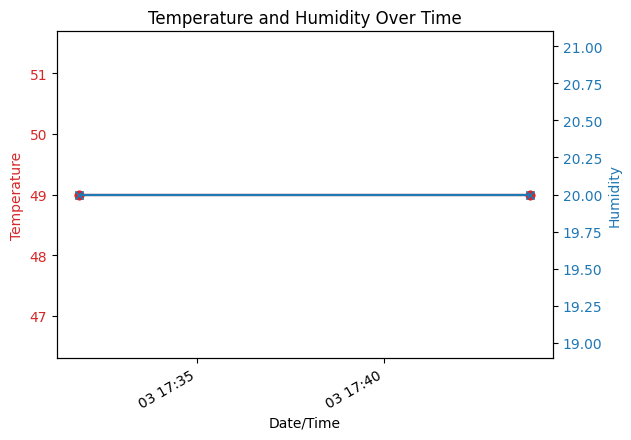
\includegraphics[width=0.5\linewidth]{Images/temp_and_humidity_over_time.png}
    \caption{Temperature and Humidity plotted overtime}
    \label{Temperature and Humidity plotted overtime}
\end{figure} 
last we tested if our code  satisfies our  python code after testing the unit test code we updated see the following message
\begin{figure}[h!]
    \centering
    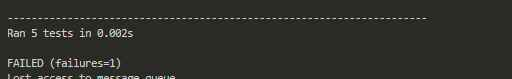
\includegraphics[width=0.5\linewidth]{Images/unit_testoutput.jpg}
    \caption{unit test message for DHT22 module}
    \label{unit test message for DHT22 module}
\end{figure}
\newpage
\subsection{AS312}
\begin{table}[h!]
    \centering
    \begin{tabular}{|c|c|}
        \hline
        date/time of record & motion detected(yes/no)\\
        \hline \hline
        2024-03-25_15-02-57&False \\
        2024-03-25_15-04-37&True\\
        2024-05-03_18-07-51&False\\
        2024-05-03_18-18-37&True
        \hline
    \end{tabular}
    \caption{Recorded data from  AS312 on the \today}
    \label{Recorded data from  AS312 on the \today}
\end{table}
\subsection{DFR0026}
For first test we got  the following table: 
\begin{table}[h!]
    \centering
    \begin{tabular}{|c|c|}
        \hline
        Date/time of record & lux values(lux)\\
        \hline \hline
        2024-03-25_15-02-57&940\\
        2024-03-25_15-03-13&945\\
        2024-03-25_15-04-37&4963\\
        2024-05-03_18-54-57&1284
        \hline
    \end{tabular}
    \caption{Recorded data from DFR0026 on the 25th of march 2024}
    \label{Recorded data from DFR0026 on the 25th of march 2024}
\end{table}
If this is plotted we get the following:
\begin{figure}[h!]
    \centering
    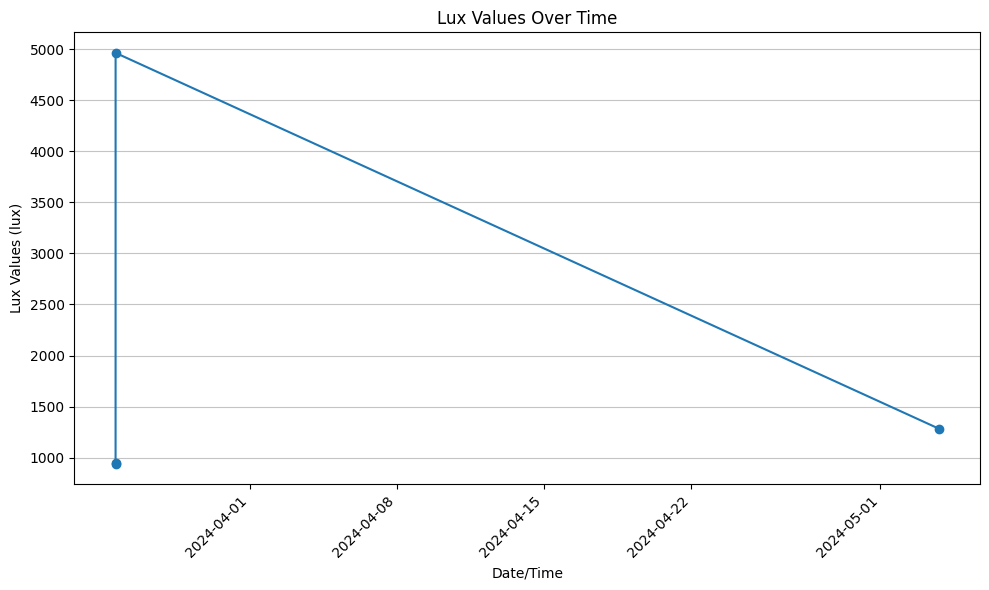
\includegraphics[width=0.5\linewidth]{Images/lux_values_overtime.png}
    \caption{lux values overtime}
    \label{lux values overtime}
\end{figure}
\newpage
\subsection{Raspberry Pi VR 220}
When testing  the Raspberry Pi VR 220 the following picture was taken:
\begin{figure}[h!]
    \centering
    
\includegraphics[width=0.4\linewidth]{Images/camera_output_2024-03-21_21-43-16.png}
    \caption{A photo from 25th of march 2024 }
    \label{A photo from 25th of march 2024}
\end{figure}

\section{Recorded data from transceiver}
When testing  the radio module the follow was tested:
\begin{enumerate}
    \item Sending a message across the serial

    \item Sending a txt file across the serial

    \item Sending a csv file across the serial


    \item Sending a image file across the serial

    none results where obtained due to  factor on \pageref{Discussion of Lora module}
\end{enumerate}
